\documentclass{amsart}
\usepackage[utf8]{inputenc}

\usepackage[parfill]{parskip}
\usepackage[dvipsnames]{xcolor}
\usepackage{microtype}
\usepackage{siunitx}
\DeclareSIUnit\year{yr}
\usepackage{pgfplots}
\usepackage{graphicx}
\usepackage{sidecap}
\sidecaptionvpos{figure}{c}
\usepackage{float}
\usepackage{gensymb}
\usepackage{tkz-euclide}
\usetkzobj{all}
\usepackage{commath}
\usepackage{hyperref}
\usepackage{enumitem}
\usepackage{wasysym}

\renewcommand*{\thefootnote}{\fnsymbol{footnote}}

\newtheorem*{thm}{Theorem}
\newtheorem*{iden}{Identity}
\newtheorem*{lemma}{Lemma}
\theoremstyle{definition}
\newtheorem*{defn}{Definition}
\newtheorem*{ex}{Example}

% russian integral
\usepackage{scalerel}
\DeclareMathOperator*{\rint}{\scalerel*{\rotatebox{17}{$\!\int\!$}}{\int}}

% \qformat{Question \thequestion: \thequestiontitle\hfill}

\begin{document}
\section*{Worked solution for problem:}
\textit{(Difficult) A cone of radius $ r $ centimetres and height $ h $ centimetres is lowered point first
            at a rate of \SI{1}{\centi\metre\squared} into a cylinder of radius $ R $ centimetres that is partially filled with
            water. How fast is the water level rising at the instant that the cone is fully submerged?}

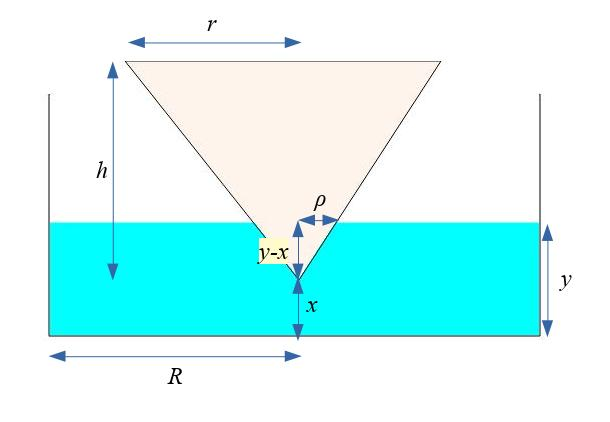
\includegraphics[width=\textwidth]{coneintank}

Let $ V $ be the volume of water in the tank, which we know to be constant. We are given that $ \od{x}{t} = -1 $. Using trigonometry,
we find $ \rho = \frac{r}{h}(y - x) $ so we have
\begin{align*}
  V &= x\pi R^2 + (y - x) \pi R^2 - \frac{1}{3} \pi \rho^2 (y-x)\\
    &= \pi R^2 y - \frac{1}{3} \pi \frac{r^2}{h^2} (y-x)^3
\end{align*}

Hence $ \od{V}{x} = \pi R^2 - \frac{\pi r^2}{h^2} (y-x)^2 (1 - \od{x}{y}) $; but $ V $ is constant, so any derivative of $ V $ is zero and
\begin{displaymath}
  0 = \pi R^2 - \frac{\pi r^2}{h^2} (y-x)^2 (1 - \od{x}{y}).
\end{displaymath}

When the cone is exactly submerged, $ y - x = h $. So $ 0 = R^2 - r^2 (1 - \od{x}{y}) $ and $ \od{x}{y} = \frac{r^2 - R^2}{r^2} $; hence
\begin{displaymath}
  \od{y}{t} = \od{x}{t} \od{y}{x} = -1 \times \frac{r^2}{r^2 - R^2} = \frac{r^2}{R^2 - r^2}.
\end{displaymath}

\end{document}
